\documentclass{beamer}
\usetheme{Boadilla}

\usepackage[T2A]{fontenc}
\usepackage[utf8]{inputenc}
\usepackage[russian]{babel}
\usepackage{mathptmx} 

\title{1297.Палиндромы}
\subtitle{Решение и разбор}
\author{Михаил Бакиновский}
\institute{БФУ имени И.Канта}
\date{\today}

\begin{document}
	\begin{frame}
	\titlepage
	\end{frame}

	\begin{frame}
		\frametitle{Содержание}
		\begin{itemize}
			\item Разбор задачи
			\begin{itemize}
				\item Исходная формулировка
				\item Разбор требований и исходных данных
			\end{itemize}
			\item Решение задачи
			\item Ссылки
		\end{itemize}
	\end{frame}
	
	\begin{frame}
		\frametitle{Разбор задачи}
		\begin{block}{Формулировка задачи}
			Найти максимальную по длине подстроку, читающуюся одинаково в обоих направлениях (палиндромы) в строке. 
			Если таких подстрок несколько, вывести из них ту, что ближе к началу строки (находится левее).
		\end{block}
		\begin{block}{Исходные данные и требования}
			\begin{itemize}
				\item Дано: Строка длины n (0<n<1001), состоящая из символов латинского алфавита без знаков препинания и пробелов.
				\item Требования: 
				\begin{itemize}
					\item Ограничение времени: 1.0 секунды
					\item Ограничение памяти: 64 МБ
				\end{itemize}
			\end{itemize}
		\end{block}
	\end{frame}

	\begin{frame}
		\frametitle{Решение задачи}
			\text{\large{\textbf{\textit{Код решения:}}}} \newline	
			(1)\text{\kern 1pc $stroke=input()$}\newline
			(2)\text{\kern 1pc $max=stroke[0]$}\newline
			(3)\text{\kern 1pc $for\,i\,in\,range(0,len(stroke)-1):$}\newline
			(4)\text{\kern 3pc $for\,j\,in\,range(len(stroke),i,-1):$}\newline
			(5)\text{\kern 5pc $comp=stroke[i:j]$}\newline
			(6)\text{\kern 5pc $if\,comp == comp[::-1]:$}\newline
		        (7)\text{\kern 7pc $if\,len(max)<len(comp):$}\newline
		        (8)\text{\kern 7pc $max=comp$}\newline
			(9)\text{\kern 1pc $print(max)$}\newline\newline
			\text{\small\textit{Использованный ЯП --- Python, версии 3.10}}
	\end{frame}

	\begin{frame}
		\frametitle{Построчное объяснение решения}
		(1) Переменная строки для работы, вводится с клавиатуры.\newline
		(2) Переменная максимального палиндрома.\newline
		(3) Главный цикл, определяющий начальную позицию подстроки.\newline
		(4) Подцикл, определяющий конечную позицию подстроки.\newline
		(5) Взятие подстроки из исходной, где i--начальная позиция среза, j--конечная.\newline
		(6) Условие равенства подстрок, где comp - подстрока, comp[::-1] -- обратная к ней.\newline
		(7) Сравнение длины палиндрома,\newline
		(8) если сохранённый меньше найденного -- сохраняем новый.\newline
		(9) На вывод получаем последний сохранённый палиндром.\newline
	\end{frame}

	\begin{frame}
		\frametitle{Ссылки}
		\begin{figure}
			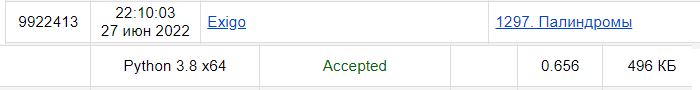
\includegraphics[scale=0.6]{accepted}
			\caption{Проверка на acm.timus.ru}
		\end{figure}
		\begin{itemize}
			\item \href{https://acm.timus.ru/}{Timus Online Judge}
			\item {GitHub ссылки
			\begin{itemize}
			\item \href{https://acm.timus.ru/}{GitHub-репозиторий}
			\item \href{https://github.com/Nelifax/Summer-practice/blob/58ef02507143101c32afc2fd39323e81d402ca8e/MVS_Python3x/practice/practice/practice.py}{GitHub-Код решения}
			\end{itemize}}
		\end{itemize}
	\end{frame}

\end{document}